\chapter{Architectures and training pipeline}
\label{chap:archi}

This chapter is the engineering counterpart of \cref{chap:theory}.
\Cref{sec:archi-cnn,sec:archi-resnet,sec:archi-attn} describe the three
neural networks we trained, with their exact layer composition and the
intent behind each design choice. \Cref{sec:archi-compare} summarises
the three in a single comparison table. \Cref{sec:archi-train} then
documents the shared training pipeline.

The three architectures are \emph{identical} between v1 and v2 ---
only the input dataset and the number of classes change. The class
count is set by the data and is the only architecture knob that
depends on it: $K = 7$ for v1, $K = 4$ for v2. All structural
parameters (channel widths, kernel sizes, attention heads, dropout)
are the same in both iterations.

The three models share the same \emph{interface}: input
$\mathbf{x} \in \R^{1 \times 512}$ (a single channel, a window of $512$
samples), output $\hat{p} \in \R^{K}$ (probabilities over the $K$
classes). This makes them drop-in interchangeable for the training and
inference scripts, which select a model by name and otherwise behave
identically.

\section{Architecture A --- baseline 1D-CNN}
\label{sec:archi-cnn}

The first model, defined in
\texttt{architectures/saved\_models/1d\_cnn.py}, is a deliberately
compact convolutional network. It serves both as a baseline to beat
and as a sanity check that the data and the training pipeline are
correctly wired.

\paragraph{Structure.} The network is a linear stack of three
convolution--BatchNorm--ReLU--MaxPool blocks, followed by an adaptive
average pool and a small classifier head:

\begin{table}[H]
    \centering
    \footnotesize
    \begin{tabular}{@{}l p{0.55\linewidth} l@{}}
        \toprule
        \textbf{Block} & \textbf{Operation} & \textbf{Output shape} \\
        \midrule
        Input       & Raw window                                                                                       & $(1, 512)$ \\
        Block 1     & $\Conv(1{\to}16, k{=}7, p{=}3) \to \BN \to \ReLU \to \mathrm{MaxPool}(2)$                          & $(16, 256)$ \\
        Block 2     & $\Conv(16{\to}32, k{=}7, p{=}3) \to \BN \to \ReLU \to \mathrm{MaxPool}(2)$                         & $(32, 128)$ \\
        Block 3     & $\Conv(32{\to}64, k{=}5, p{=}2) \to \BN \to \ReLU \to \mathrm{MaxPool}(2)$                         & $(64, 64)$ \\
        Pool        & $\mathrm{AdaptiveAvgPool1d}(4)$                                                                  & $(64, 4)$ \\
        Classifier  & $\mathrm{Flatten} \to \mathrm{Dropout}(0.4) \to \mathrm{Linear}(256{\to}32) \to \ReLU \to \mathrm{Dropout}(0.2) \to \mathrm{Linear}(32{\to}K)$ & $(K)$ \\
        \bottomrule
    \end{tabular}
\end{table}

\paragraph{Design notes.}
\begin{itemize}[leftmargin=*, itemsep=0.2em]
    \item Kernel sizes $k=7,7,5$ are large enough to capture multi-sample
    shape primitives at each scale while staying well within the
    receptive-field budget.
    \item Channel widths $16 \to 32 \to 64$ double at each block,
    compensating the temporal compression by a factor of $2$ at every
    \texttt{MaxPool}.
    \item \texttt{AdaptiveAvgPool1d(4)} keeps four temporal bins after
    the convolutional trunk: this preserves a coarse notion of
    ``where in the window the activation peaks'', useful for shapes
    such as \texttt{fast\_ascend} vs \texttt{fast\_descend} that differ
    mainly by the location of their peak.
    \item Two dropout layers ($p=0.4$ then $p=0.2$) in the
    fully-connected head act as a regulariser.
\end{itemize}

Total trainable parameters: $22\,727$ (v1, $K = 7$) /
$22\,628$ (v2, $K = 4$). The classifier head's output width is the
only thing that changes between the two iterations.

\section{Architecture B --- 1D Residual Network}
\label{sec:archi-resnet}

The second model, defined in
\texttt{architectures/saved\_models/resNet.py}, replaces each
convolutional block of model A with a small \emph{residual block}
(\cref{sec:resnet-theory}) and substitutes every BatchNorm with
GroupNorm (\cref{sec:gn-theory}).

\paragraph{Residual block.} A single block transforms an input of
channel count $c_{\text{in}}$ into an output of channel count
$c_{\text{out}}$ as
\begin{align*}
    \mathcal{F}(\mathbf{u}) &= \mathrm{GN} \!\circ\! \Conv_{k_3} \!\circ\! \ReLU \!\circ\! \mathrm{GN} \!\circ\! \Conv_{k_2} \!\circ\! \ReLU \!\circ\! \mathrm{GN} \!\circ\! \Conv_{k_1} (\mathbf{u}), \\
    \text{Block}(\mathbf{u}) &= \ReLU\bigl( \mathcal{F}(\mathbf{u}) + \mathrm{Shortcut}(\mathbf{u}) \bigr),
\end{align*}
where the shortcut is either the identity (when $c_{\text{in}} =
c_{\text{out}}$) or a $1{\times}1$ convolution followed by GroupNorm.
Kernel sizes $(k_1, k_2, k_3)$ are $(15, 9, 5)$ in the first block
(broad context immediately) and $(7, 5, 3)$ in the next two.

\paragraph{Full structure.}

\begin{table}[H]
    \centering
    \footnotesize
    \begin{tabular}{@{}l p{0.55\linewidth} l@{}}
        \toprule
        \textbf{Block} & \textbf{Operation} & \textbf{Output shape} \\
        \midrule
        Input       & Raw window                                                              & $(1, 512)$ \\
        Block 1     & $\mathrm{Res}\bigl( 1 \to 16, \, k{=}(15,9,5) \bigr)$                   & $(16, 512)$ \\
        Pool 1      & $\mathrm{MaxPool}(2)$                                                   & $(16, 256)$ \\
        Block 2     & $\mathrm{Res}\bigl( 16 \to 32, \, k{=}(7,5,3) \bigr)$                   & $(32, 256)$ \\
        Pool 2      & $\mathrm{MaxPool}(2)$                                                   & $(32, 128)$ \\
        Block 3     & $\mathrm{Res}\bigl( 32 \to 64, \, k{=}(7,5,3) \bigr)$                   & $(64, 128)$ \\
        Pool        & $\mathrm{AdaptiveAvgPool1d}(4)$                                          & $(64, 4)$ \\
        Classifier  & Same head as model A                                                    & $(K)$ \\
        \bottomrule
    \end{tabular}
\end{table}

\paragraph{Design notes.}
\begin{itemize}[leftmargin=*, itemsep=0.2em]
    \item GroupNorm with $\min(8, c_{\text{out}})$ groups everywhere
    means train-time and inference-time behaviour are identical, which
    matters when deploying on real data with a different value
    distribution.
    \item The shortcut connections preserve the original signal
    through the convolutional trunk, allowing later blocks to focus on
    \emph{adding} discriminative information.
    \item The classifier head is intentionally identical to that of
    model A so that the residual trunk is the only difference between
    the two networks --- a clean ablation.
\end{itemize}

Total trainable parameters: $74\,631$ (v1) / $74\,532$ (v2).

\section{Architecture C --- CNN+Attention}
\label{sec:archi-attn}

The third model, defined in
\texttt{architectures/saved\_models/cnn\_attention.py}, hybridises a
convolutional stem with a Transformer encoder
(\cref{sec:encoder-theory}). The motivation is to combine the
\emph{locality} of convolutions, well-suited to short shape primitives,
with the \emph{global mixing} of attention, which lets the network
reason about how those primitives compose over the whole window.

\paragraph{Convolutional stem.}
Three Conv--GroupNorm--ReLU blocks reduce the temporal length by a
factor of $8$ via stride-$2$ convolutions:

\begin{table}[H]
    \centering
    \footnotesize
    \begin{tabular}{@{}l p{0.55\linewidth} l@{}}
        \toprule
        \textbf{Layer} & \textbf{Operation} & \textbf{Output shape} \\
        \midrule
        Input  & Raw window                                                                  & $(1, 512)$ \\
        Stem 1 & $\Conv(1{\to}16, k{=}7, s{=}2, p{=}3) \to \mathrm{GN}(8) \to \ReLU$           & $(16, 256)$ \\
        Stem 2 & $\Conv(16{\to}32, k{=}5, s{=}2, p{=}2) \to \mathrm{GN}(8) \to \ReLU$          & $(32, 128)$ \\
        Stem 3 & $\Conv(32{\to}64, k{=}3, s{=}2, p{=}1) \to \mathrm{GN}(8) \to \ReLU$          & $(64, 64)$ \\
        \bottomrule
    \end{tabular}
\end{table}

\paragraph{Tokenisation and Transformer encoder.}
The stem output is reshaped to a sequence of $T = 64$ tokens of
dimension $d = 64$. A learnable $\texttt{[CLS]}$ token is prepended
($T' = 65$ tokens total), a sinusoidal positional encoding
(\cref{eq:posenc}) is added, and two pre-LayerNorm encoder blocks are
applied. Each encoder block has $h = 4$ attention heads of dimension
$d_h = 16$ and a feed-forward network with hidden size
$d_{\mathrm{ff}} = 4 d = 256$, GELU activation and dropout $p = 0.1$.

\paragraph{Classification.}
The encoder output at the $\texttt{[CLS]}$ position is
LayerNorm-normalised and passed through a single linear layer
$\R^{d} \to \R^{K}$ to produce the class logits.

\paragraph{Design notes.}
\begin{itemize}[leftmargin=*, itemsep=0.2em]
    \item The stride-$2$ convolutional stem reduces the sequence length
    eightfold before attention, keeping the $O(T^2)$ cost of attention
    manageable at $65^2 \approx 4\,000$ pairs.
    \item GroupNorm (not BatchNorm) in the stem makes the entire
    feature extraction amplitude-invariant on a per-window basis ---
    consistent with the window-mean centring of \cref{eq:window-norm}.
    \item The $\texttt{[CLS]}$ token is initialised with a small random
    vector (truncated normal, $\sigma = 0.02$) and is the only
    \emph{learnable} positional information; the sinusoidal encoding
    is shared and fixed.
\end{itemize}

Total trainable parameters: $109\,655$ (v1) / $109\,460$ (v2).

\section{Side-by-side comparison}
\label{sec:archi-compare}

\Cref{tab:archi-compare} summarises the three architectures.

\begin{table}[H]
    \centering
    \footnotesize
    \begin{tabular}{lccc}
        \toprule
        & \textbf{1D-CNN} & \textbf{ResNet 1D} & \textbf{CNN+Attention} \\
        \midrule
        Convolutional trunk         & 3 plain blocks & 3 residual blocks & 3-layer stride-2 stem \\
        Normalisation               & BatchNorm      & GroupNorm(8)      & GroupNorm(8) \\
        Skip connections            & ---            & yes               & yes (inside Transformer) \\
        Long-range mixing           & ---            & ---               & Multi-head self-attention \\
        Output head                 & MLP(256\,$\to$\,32\,$\to$\,K) & MLP(256\,$\to$\,32\,$\to$\,K) & Linear(64\,$\to$\,K) on CLS \\
        Trainable parameters (v2)   & $22\,628$      & $74\,532$         & $109\,460$ \\
        \bottomrule
    \end{tabular}
    \caption{Side-by-side summary of the three architectures.}
    \label{tab:archi-compare}
\end{table}

\section{Training pipeline}
\label{sec:archi-train}

The training pipeline is implemented once, in
\texttt{architectures/train.py}, and parameterised by the model name.

\subsection{Data preparation}

The raw signal is split temporally (80/20) into a train+val pool and a
test pool (\cref{sec:split-theory}), then converted into sliding
windows of size $512$ with stride $32$. The temporal split before
windowing is what protects against data leakage between train and
test windows.

\paragraph{Windowing.} Each window is centred individually (subtract
its own mean) and scaled by the global training standard deviation
$\sigma_{\text{train}}$, which is saved in a JSON file next to the
model weights so that inference uses exactly the same scaling.

\begin{figure}[H]
    \centering
    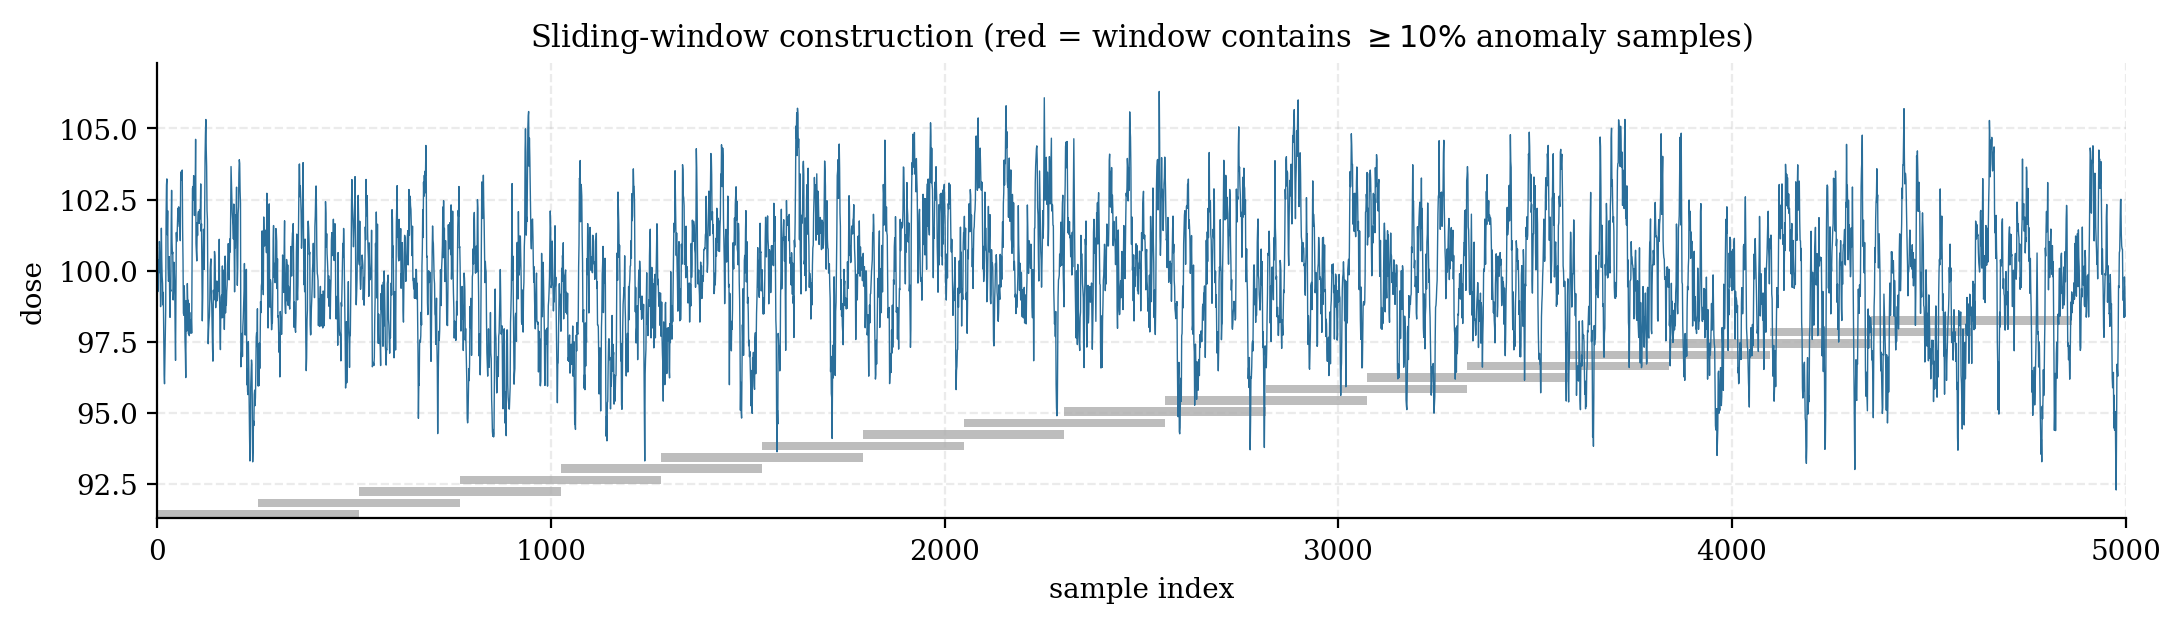
\includegraphics[width=0.95\linewidth]{figures/sliding_window}
    \caption{Sliding-window construction on a fragment of the v2
    synthetic signal. Each coloured bar represents one $512$-sample
    training window; red bars indicate windows that capture
    $\geq 30\%$ of an underlying event's samples and so inherit its
    class label (event-coverage rule, \cref{sec:framing}).}
    \label{fig:sliding-window}
\end{figure}

\subsection{Optimisation}

All three models are trained with the recipe of
\cref{sec:train-theory}: Adam ($\eta = 10^{-3}$, default
$\beta_1, \beta_2$), batch size $128$, weighted cross-entropy
\cref{eq:cross-entropy}, a $\texttt{ReduceLROnPlateau}$ scheduler with
patience $2$ and factor $0.5$, early stopping with patience $10$ and
minimum delta $5 \cdot 10^{-3}$, maximum $35$ epochs. No data
augmentation is applied --- the stochastic anomaly generation already
provides enough variability.

\subsection{Class-weighting in v1 vs v2}

The two iterations differ markedly in their training class
distribution, and therefore in the class-weight vector that the loss
uses (\cref{fig:failure-analysis}).

\begin{figure}[H]
    \centering
    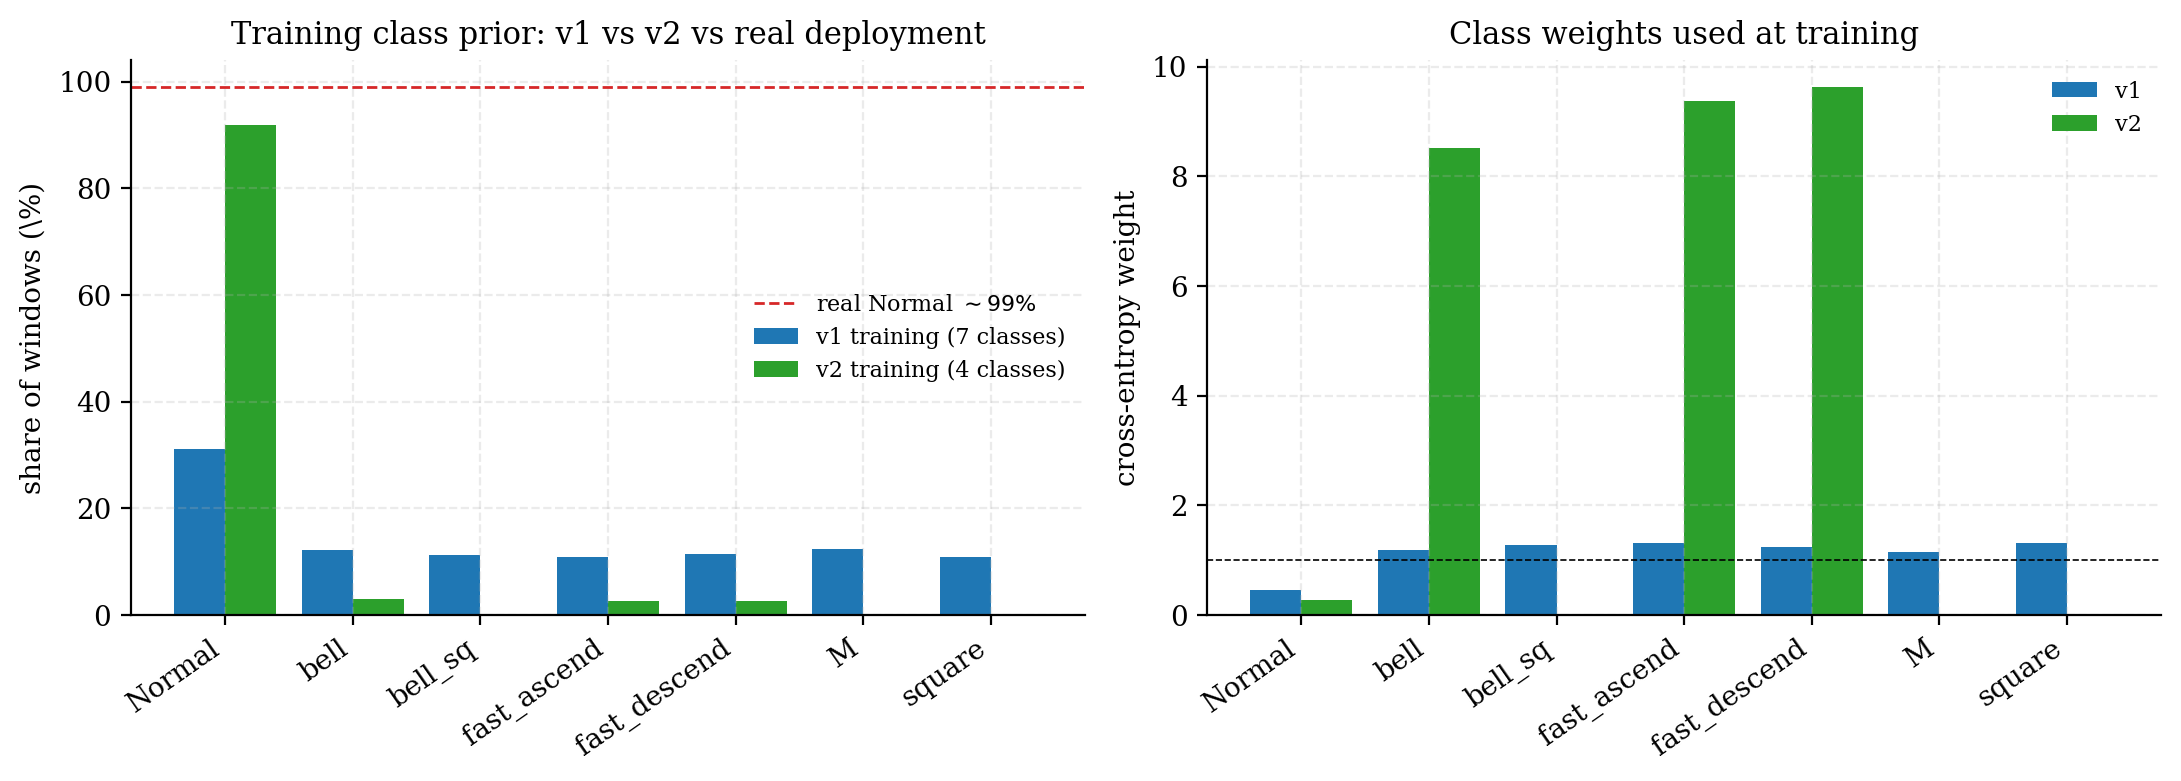
\includegraphics[width=\linewidth]{figures/failure_analysis}
    \caption{\textbf{Left}: window-level class distribution at training,
    for v1 (seven classes, blue) and v2 (four classes, green), against
    the (estimated) real deployment prior in red ($\sim 99\%$
    \texttt{Normal}). v1 has been trained with a prior that is roughly
    the \emph{opposite} of the deployment prior. v2 closes the gap to
    within a factor of three. \textbf{Right}: cross-entropy class
    weights used in each iteration. v2 strongly down-weights
    \texttt{Normal} ($w_0 = 0.27$ vs $\sim 9$ on the anomaly classes)
    because the class imbalance in v2 is also much larger than in v1.}
    \label{fig:failure-analysis}
\end{figure}

\paragraph{v1 class weights.} v1 has $\sim 31\%$ \texttt{Normal} and
$\sim 11\%$ per anomaly class, yielding weights
$\mathbf{w}_{\text{v1}} = (0.46, 1.18, 1.27, 1.32, 1.24, 1.15, 1.31)$.

\paragraph{v2 class weights.} v2 has $\sim 92\%$ \texttt{Normal} and
$\sim 3\%$ per anomaly class, yielding weights
$\mathbf{w}_{\text{v2}} = (0.27, 8.51, 9.37, 9.63)$.

\subsection{Selection criterion}

The training script saves the weights with the lowest validation loss.
Validation F1 score (macro-averaged across the classes) is tracked at
every epoch for diagnostic purposes but is not used for selection.
